\documentclass{beamer}

%encoding
%--------------------------------------
\usepackage[T1]{fontenc}
\usepackage[utf8]{inputenc}
%--------------------------------------

%Portuguese-specific commands
%--------------------------------------
\usepackage[portuguese]{babel}
%--------------------------------------

\usepackage{tikz}
\usepackage{pgfplots}
\pgfplotsset{compat = newest}
\usepgfplotslibrary{colormaps}

%Hyphenation rules
%--------------------------------------
\usepackage{hyphenat}
\hyphenation{mate-mática recu-perar}
%--------------------------------------

\usepackage{wrapfig}
\usepackage{graphicx}
\usepackage{biblatex}
\usepackage[document]{ragged2e}

%\DeclareCaptionFormat{myformat}{\fontsize{4}{5}\selectfont#1#2#3}
\usepackage[font=scriptsize,labelformat=empty,labelfont=it,textfont=it]{caption}
 \def\vec{\mathaccent "017E\relax }

%\captionsetup[figure]{format=myformat, labelformat=empty} 

% \usepackage[
% backend=biber,
% style=alphabetic,
% sorting=ynt
% ]{biblatex}
\addbibresource{latex-beamer-template.bib}

\graphicspath{ {../../images/} {.images} }

% \usefonttheme{structuresmallcapsserif}
\usetheme{Warsaw}
% \usecolortheme{beetle}
\usecolortheme{seagull}

% \setbeamertemplate{navigation symbols}{}
% \setbeamertemplate{mini frames}{}
\setbeamertemplate{headline}{}
% \renewcommand*{\slideentry}[6]{}
\setbeamertemplate{section in toc}[sections numbered]
\setbeamertemplate{subsection in toc}[subsections numbered]

\setbeamercolor{block body}{bg=yellow!30}
\setbeamercolor{block title}{bg=yellow!40}

\setbeamercolor{block body alerted}{bg=red!10}
\setbeamercolor{block title alerted}{bg=red!20}

\setbeamercolor{block body example}{bg=green!10}
\setbeamercolor{block title example}{bg=green!20}

% Information to be included in the title page:
\title{A Independência do Caminho na Integral do Trabalho}
\subtitle{Trabalho 1 - Grupo 16}

\author [Alex, Caio, Pedro]{
    \small Alex Campbell e Souza - Engenharia de Sistemas \\ 
    Caio Lucas Gomes Silva - Matemática \\ 
    Pedro Mansur Gamarano - Matemática
}

\institute[]{
    \large UFMG \\
    \footnotesize Universidade Federal de Minas Gerais \\
    \small Fundamentos de Eletromagnetismo
}


\date{\today}

\begin{document}

% Slide inicial com título
\frame{\titlepage}

% Índice
%\begin{frame}
%    \frametitle{Index}
\frame{\tableofcontents}
%\end{frame}

% Exibido, no começo de cada seção, o tópico corrente
% \AtBeginSection[]
% {
%   \begin{frame}
%     \frametitle{New Topic}
%     \tableofcontents[currentsection]
%   \end{frame}
% }
\section{Introdução}
\begin{frame}
    \frametitle{O Trabalho (W)}
    
    O trabalho é a grandeza física associada a mudança de energia. 
    Ele acontece quando aplicamos uma força sobre um corpo e este sofre um deslocamento. 
    O trabalho de uma força constante pode ser escrito como: 
    \begin{equation}\label{eq:trabalho-constante}
    W = F * d * cos(\theta)
    \end{equation}

    Já o trabalho de uma força não constante pode ser escrito como: 
    \begin{equation}\label{trabalho-nao-constante}
    W = \mathit{\int_{a}^b \vec{F} d\vec{r}}
    \end{equation}
%     \begin{tikzpicture}
%         \begin{axis}[
%         xmin = -4, xmax = 4,
%         ymin = -4, ymax = 4,
%         zmin = 0, zmax = 1,
%         axis equal image,
%         xtick distance = 1,
%         ytick distance = 1,
%         view = {0}{90},
%         scale = 1.25,
%         colormap/viridis,
%         colorbar,
%         colorbar style = {
%         ylabel = {Vector Length}
%         }
%         ]
%         \addplot3[
%         point meta = {sqrt(x^2+y^2)},
%         quiver = {
%         u = {-y/sqrt(x^2+y^2)},
%         v = {x/sqrt(x^2+y^2)},
%         scale arrows = 0.25,
%         },
%         quiver/colored = {mapped color},
%         -stealth,
%         domain = -4:4,
%         domain y = -4:4,
%         ] {0};
%         \end{axis}
%     \end{tikzpicture}
%\end{frame}

% \begin{frame}
%     \frametitle{About me}
%     \begin{wrapfigure}{r}{0.25\textwidth} %this figure will be at the right
%         \centering
%         \caption{My picture. =)}
%         
\includegraphics[width=0.25\textwidth]{avatar.jpeg}
%         \label{fig:avatar}
%     \end{wrapfigure}
% 
%     Lorem ipsum dolor sit amet, consectetur adipiscing elit.
% 
%     Curabitur eget tortor at quam ullamcorper pellentesque.
%     Morbi ac enim eu ante viverra elementum id viverra justo.
%     Mauris sagittis mauris sed laoreet maximus. 
%     \cite{dirac}
% 
% %    \begin{figure}[h]
% %        \caption{That's me. =)}
% %        
\includegraphics[width=0.5\textwidth, scale=0.25]{avatar.jpeg}
% %    \end{faigure}
% 
%     \listoffigures
% 
\end{frame}
% 
%\section{sec-2}

\begin{frame}
    \frametitle{Campos Elétricos e Campos Conservativos}
    
    O \textbf{método da idependência do caminho} é possivel apenas em campos conservativos. 
    Um campo é conservativo quando ele é obtido atraves do cálculo do vetor gradiente de uma função. 
    O campo elétrico é um exemplo de campo conservativo.
    
%    \begin{figure}
%    $$
%        \mathit{\int_{a}^b \vec{F} d\vec{r}}
%    $$
%    \caption{Trabalho realizado por uma força $\vec{F}$ ao longo de $\vec{r}$}\label{fig:1}
%    \end{figure}

\end{frame}

\begin{frame}
    \frametitle{Campos Elétricos e Campos Conservativos}
    
    
    \begin{wrapfigure}{r}{0.4\textwidth} %this figure will be at the right
        \vspace{-35pt}
        \centering
        \caption{}
        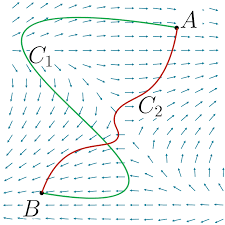
\includegraphics[width=0.30\textwidth]{grafico-trabalho.png}
        \label{fig:grafico-trabalho}
    \end{wrapfigure}
    
    A \textbf{independencia do caminho} diz que, em campos conservativos, quaisquer integrais de 
    linha que possuemos mesmos pontos inicial e final resultam em um mesmo valor, independente da curva entre eles. 
    Utilizando o trabalho como exemplo:  
    \hfill \break
    \hfill \break
    %\begin{equation}\label{trabalho-nao-constante}
    $    
        W = \mathit{\int_{c_1} \vec{F} d\vec{r}} = f(b) - f(a) 
        \hfill \break
        W = \mathit{\int_{c_2} \vec{F} d\vec{r}} = f(b) - f(a) 
    $
    %\end{equation}

\end{frame}


% \begin{frame}
%     \begin{tikzpicture}
%         \begin{axis}[
%         xmin = -10, xmax = 10,
%         ymin = -10, ymax = 10,
%         zmin = 0, zmax = 1,
%         axis equal image,
%         xtick distance = 2,
%         ytick distance = 2,
%         view = {0}{100},
%         scale = 0.75,
%         colormap/viridis
%         ]
%         \addplot3[
%         point meta = {sqrt(x^2+y^2)},
%         quiver = {
%         u = {x^2/( 1 - t^2, t )},
%         v = {\cos(y)/( 1 - t^2, t )},
%         scale arrows = 1,
%         },
%         quiver/colored = {mapped color},
%         -stealth,
%         domain = -10:10,
%         domain y = -10:10,
%         ] {0};
%         \end{axis}
% \end{tikzpicture}
% \end{frame}

\section{Exemplos}

\begin{frame}
    \frametitle{Exemplo 1} 

    \begin{wrapfigure}{r}{0.4\textwidth} %this figure will be at the right
        \vspace{-35pt}
        \centering
        \caption{}
        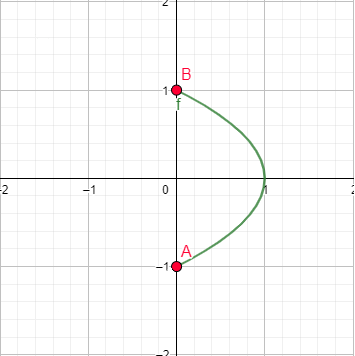
\includegraphics[width=0.30\textwidth]{grafico-exemplo-1.png}
        \label{fig:grafico-exemplo1}
    \end{wrapfigure}

    Dado o campo conservativo $ F(x, y) = ( x^2, \cos(y) ) $, calcule o trabalho de deslocamento sobre a 
    curva $ c_1(t) = ( 1 - t^2, t ) $ que tem ponto inicial $ A( 0, -1) $ e final $ B( 0, 1) $ [ -1, 1 ].

    $
        \int{} \vec{F} d\vec{r} =  
        \begin{cases}
            x(n),\\
            x(n-1)\\
            x(n-1)
        \end{cases}
    $
%     In this slide, some important text will be
%     \alert{highlighted} because it's important.
%     Please, don't abuse it.
%     
%     \begin{block}{Genérico}
%     Bloco ``Genérico"
%     \end{block}
%     
%     \begin{alertblock}{Importante}
%     Bloco amarelo para ``Atenção".
%     \end{alertblock}
%     
%     \begin{examples}{Boas Práticas}
%     Bloco verde para ``Boas Práticas".
%     \end{examples}

\end{frame}

\frame{\printbibliography}

\end{document}